
%% bare_conf.tex
%% V1.3
%% 2007/01/11
%% by Michael Shell
%% See:
%% http://www.michaelshell.org/
%% for current contact information.
%%
%% This is a skeleton file demonstrating the use of IEEEtran.cls
%% (requires IEEEtran.cls version 1.7 or later) with an IEEE conference paper.
%%
%% Support sites:
%% http://www.michaelshell.org/tex/ieeetran/
%% http://www.ctan.org/tex-archive/macros/latex/contrib/IEEEtran/
%% and
%% http://www.ieee.org/

%%*************************************************************************
%% Legal Notice:
%% This code is offered as-is without any warranty either expressed or
%% implied; without even the implied warranty of MERCHANTABILITY or
%% FITNESS FOR A PARTICULAR PURPOSE!
%% User assumes all risk.
%% In no event shall IEEE or any contributor to this code be liable for
%% any damages or losses, including, but not limited to, incidental,
%% consequential, or any other damages, resulting from the use or misuse
%% of any information contained here.
%%
%% All comments are the opinions of their respective authors and are not
%% necessarily endorsed by the IEEE.
%%
%% This work is distributed under the LaTeX Project Public License (LPPL)
%% ( http://www.latex-project.org/ ) version 1.3, and may be freely used,
%% distributed and modified. A copy of the LPPL, version 1.3, is included
%% in the base LaTeX documentation of all distributions of LaTeX released
%% 2003/12/01 or later.
%% Retain all contribution notices and credits.
%% ** Modified files should be clearly indicated as such, including  **
%% ** renaming them and changing author support contact information. **
%%
%% File list of work: IEEEtran.cls, IEEEtran_HOWTO.pdf, bare_adv.tex,
%%                    bare_conf.tex, bare_jrnl.tex, bare_jrnl_compsoc.tex
%%*************************************************************************

% *** Authors should verify (and, if needed, correct) their LaTeX system  ***
% *** with the testflow diagnostic prior to trusting their LaTeX platform ***
% *** with production work. IEEE's font choices can trigger bugs that do  ***
% *** not appear when using other class files.                            ***
% The testflow support page is at:
% http://www.michaelshell.org/tex/testflow/



% Note that the a4paper option is mainly intended so that authors in
% countries using A4 can easily print to A4 and see how their papers will
% look in print - the typesetting of the document will not typically be
% affected with changes in paper size (but the bottom and side margins will).
% Use the testflow package mentioned above to verify correct handling of
% both paper sizes by the user's LaTeX system.
%
% Also note that the "draftcls" or "draftclsnofoot", not "draft", option
% should be used if it is desired that the figures are to be displayed in
% draft mode.
%
\documentclass[conference]{IEEEtran}
% Add the compsoc option for Computer Society conferences.
%
% If IEEEtran.cls has not been installed into the LaTeX system files,
% manually specify the path to it like:
% \documentclass[conference]{../sty/IEEEtran}


\makeatletter
\def\ps@headings{%
\def\@oddhead{\mbox{}\scriptsize\rightmark \hfil \thepage}%
\def\@evenhead{\scriptsize\thepage \hfil \leftmark\mbox{}}%
\def\@oddfoot{}%
\def\@evenfoot{}}
\makeatother

\pagestyle{headings}
\usepackage{amsfonts}
\usepackage{amsthm}
\usepackage{amssymb}
\usepackage{amsmath}
\usepackage{graphicx}
\usepackage{fancyhdr}

\newtheorem{Prop}{Proposition}
\newtheorem{lemma}{Lemma}
\newtheorem{theorem}{Theorem}


% Some very useful LaTeX packages include:
% (uncomment the ones you want to load)


% *** MISC UTILITY PACKAGES ***
%
%\usepackage{ifpdf}
% Heiko Oberdiek's ifpdf.sty is very useful if you need conditional
% compilation based on whether the output is pdf or dvi.
% usage:
% \ifpdf
%   % pdf code
% \else
%   % dvi code
% \fi
% The latest version of ifpdf.sty can be obtained from:
% http://www.ctan.org/tex-archive/macros/latex/contrib/oberdiek/
% Also, note that IEEEtran.cls V1.7 and later provides a builtin
% \ifCLASSINFOpdf conditional that works the same way.
% When switching from latex to pdflatex and vice-versa, the compiler may
% have to be run twice to clear warning/error messages.






% *** CITATION PACKAGES ***
%
%\usepackage{cite}
% cite.sty was written by Donald Arseneau
% V1.6 and later of IEEEtran pre-defines the format of the cite.sty package
% \cite{} output to follow that of IEEE. Loading the cite package will
% result in citation numbers being automatically sorted and properly
% "compressed/ranged". e.g., [1], [9], [2], [7], [5], [6] without using
% cite.sty will become [1], [2], [5]--[7], [9] using cite.sty. cite.sty's
% \cite will automatically add leading space, if needed. Use cite.sty's
% noadjust option (cite.sty V3.8 and later) if you want to turn this off.
% cite.sty is already installed on most LaTeX systems. Be sure and use
% version 4.0 (2003-05-27) and later if using hyperref.sty. cite.sty does
% not currently provide for hyperlinked citations.
% The latest version can be obtained at:
% http://www.ctan.org/tex-archive/macros/latex/contrib/cite/
% The documentation is contained in the cite.sty file itself.






% *** GRAPHICS RELATED PACKAGES ***
%
\ifCLASSINFOpdf
  % \usepackage[pdftex]{graphicx}
  % declare the path(s) where your graphic files are
  % \graphicspath{{../pdf/}{../jpeg/}}
  % and their extensions so you won't have to specify these with
  % every instance of \includegraphics
  % \DeclareGraphicsExtensions{.pdf,.jpeg,.png}
\else
  % or other class option (dvipsone, dvipdf, if not using dvips). graphicx
  % will default to the driver specified in the system graphics.cfg if no
  % driver is specified.
  % \usepackage[dvips]{graphicx}
  % declare the path(s) where your graphic files are
  % \graphicspath{{../eps/}}
  % and their extensions so you won't have to specify these with
  % every instance of \includegraphics
  % \DeclareGraphicsExtensions{.eps}
\fi
% graphicx was written by David Carlisle and Sebastian Rahtz. It is
% required if you want graphics, photos, etc. graphicx.sty is already
% installed on most LaTeX systems. The latest version and documentation can
% be obtained at:
% http://www.ctan.org/tex-archive/macros/latex/required/graphics/
% Another good source of documentation is "Using Imported Graphics in
% LaTeX2e" by Keith Reckdahl which can be found as epslatex.ps or
% epslatex.pdf at: http://www.ctan.org/tex-archive/info/
%
% latex, and pdflatex in dvi mode, support graphics in encapsulated
% postscript (.eps) format. pdflatex in pdf mode supports graphics
% in .pdf, .jpeg, .png and .mps (metapost) formats. Users should ensure
% that all non-photo figures use a vector format (.eps, .pdf, .mps) and
% not a bitmapped formats (.jpeg, .png). IEEE frowns on bitmapped formats
% which can result in "jaggedy"/blurry rendering of lines and letters as
% well as large increases in file sizes.
%
% You can find documentation about the pdfTeX application at:
% http://www.tug.org/applications/pdftex





% *** MATH PACKAGES ***
%
%\usepackage[cmex10]{amsmath}
% A popular package from the American Mathematical Society that provides
% many useful and powerful commands for dealing with mathematics. If using
% it, be sure to load this package with the cmex10 option to ensure that
% only type 1 fonts will utilized at all point sizes. Without this option,
% it is possible that some math symbols, particularly those within
% footnotes, will be rendered in bitmap form which will result in a
% document that can not be IEEE Xplore compliant!
%
% Also, note that the amsmath package sets \interdisplaylinepenalty to 10000
% thus preventing page breaks from occurring within multiline equations. Use:
%\interdisplaylinepenalty=2500
% after loading amsmath to restore such page breaks as IEEEtran.cls normally
% does. amsmath.sty is already installed on most LaTeX systems. The latest
% version and documentation can be obtained at:
% http://www.ctan.org/tex-archive/macros/latex/required/amslatex/math/





% *** SPECIALIZED LIST PACKAGES ***
%
%\usepackage{algorithmic}
% algorithmic.sty was written by Peter Williams and Rogerio Brito.
% This package provides an algorithmic environment fo describing algorithms.
% You can use the algorithmic environment in-text or within a figure
% environment to provide for a floating algorithm. Do NOT use the algorithm
% floating environment provided by algorithm.sty (by the same authors) or
% algorithm2e.sty (by Christophe Fiorio) as IEEE does not use dedicated
% algorithm float types and packages that provide these will not provide
% correct IEEE style captions. The latest version and documentation of
% algorithmic.sty can be obtained at:
% http://www.ctan.org/tex-archive/macros/latex/contrib/algorithms/
% There is also a support site at:
% http://algorithms.berlios.de/index.html
% Also of interest may be the (relatively newer and more customizable)
% algorithmicx.sty package by Szasz Janos:
% http://www.ctan.org/tex-archive/macros/latex/contrib/algorithmicx/




% *** ALIGNMENT PACKAGES ***
%
%\usepackage{array}
% Frank Mittelbach's and David Carlisle's array.sty patches and improves
% the standard LaTeX2e array and tabular environments to provide better
% appearance and additional user controls. As the default LaTeX2e table
% generation code is lacking to the point of almost being broken with
% respect to the quality of the end results, all users are strongly
% advised to use an enhanced (at the very least that provided by array.sty)
% set of table tools. array.sty is already installed on most systems. The
% latest version and documentation can be obtained at:
% http://www.ctan.org/tex-archive/macros/latex/required/tools/


%\usepackage{mdwmath}
%\usepackage{mdwtab}
% Also highly recommended is Mark Wooding's extremely powerful MDW tools,
% especially mdwmath.sty and mdwtab.sty which are used to format equations
% and tables, respectively. The MDWtools set is already installed on most
% LaTeX systems. The lastest version and documentation is available at:
% http://www.ctan.org/tex-archive/macros/latex/contrib/mdwtools/


% IEEEtran contains the IEEEeqnarray family of commands that can be used to
% generate multiline equations as well as matrices, tables, etc., of high
% quality.


%\usepackage{eqparbox}
% Also of notable interest is Scott Pakin's eqparbox package for creating
% (automatically sized) equal width boxes - aka "natural width parboxes".
% Available at:
% http://www.ctan.org/tex-archive/macros/latex/contrib/eqparbox/





% *** SUBFIGURE PACKAGES ***
%\usepackage[tight,footnotesize]{subfigure}
% subfigure.sty was written by Steven Douglas Cochran. This package makes it
% easy to put subfigures in your figures. e.g., "Figure 1a and 1b". For IEEE
% work, it is a good idea to load it with the tight package option to reduce
% the amount of white space around the subfigures. subfigure.sty is already
% installed on most LaTeX systems. The latest version and documentation can
% be obtained at:
% http://www.ctan.org/tex-archive/obsolete/macros/latex/contrib/subfigure/
% subfigure.sty has been superceeded by subfig.sty.



%\usepackage[caption=false]{caption}
%\usepackage[font=footnotesize]{subfig}
% subfig.sty, also written by Steven Douglas Cochran, is the modern
% replacement for subfigure.sty. However, subfig.sty requires and
% automatically loads Axel Sommerfeldt's caption.sty which will override
% IEEEtran.cls handling of captions and this will result in nonIEEE style
% figure/table captions. To prevent this problem, be sure and preload
% caption.sty with its "caption=false" package option. This is will preserve
% IEEEtran.cls handing of captions. Version 1.3 (2005/06/28) and later
% (recommended due to many improvements over 1.2) of subfig.sty supports
% the caption=false option directly:
%\usepackage[caption=false,font=footnotesize]{subfig}
%
% The latest version and documentation can be obtained at:
% http://www.ctan.org/tex-archive/macros/latex/contrib/subfig/
% The latest version and documentation of caption.sty can be obtained at:
% http://www.ctan.org/tex-archive/macros/latex/contrib/caption/




% *** FLOAT PACKAGES ***
%
%\usepackage{fixltx2e}
% fixltx2e, the successor to the earlier fix2col.sty, was written by
% Frank Mittelbach and David Carlisle. This package corrects a few problems
% in the LaTeX2e kernel, the most notable of which is that in current
% LaTeX2e releases, the ordering of single and double column floats is not
% guaranteed to be preserved. Thus, an unpatched LaTeX2e can allow a
% single column figure to be placed prior to an earlier double column
% figure. The latest version and documentation can be found at:
% http://www.ctan.org/tex-archive/macros/latex/base/



%\usepackage{stfloats}
% stfloats.sty was written by Sigitas Tolusis. This package gives LaTeX2e
% the ability to do double column floats at the bottom of the page as well
% as the top. (e.g., "\begin{figure*}[!b]" is not normally possible in
% LaTeX2e). It also provides a command:
%\fnbelowfloat
% to enable the placement of footnotes below bottom floats (the standard
% LaTeX2e kernel puts them above bottom floats). This is an invasive package
% which rewrites many portions of the LaTeX2e float routines. It may not work
% with other packages that modify the LaTeX2e float routines. The latest
% version and documentation can be obtained at:
% http://www.ctan.org/tex-archive/macros/latex/contrib/sttools/
% Documentation is contained in the stfloats.sty comments as well as in the
% presfull.pdf file. Do not use the stfloats baselinefloat ability as IEEE
% does not allow \baselineskip to stretch. Authors submitting work to the
% IEEE should note that IEEE rarely uses double column equations and
% that authors should try to avoid such use. Do not be tempted to use the
% cuted.sty or midfloat.sty packages (also by Sigitas Tolusis) as IEEE does
% not format its papers in such ways.





% *** PDF, URL AND HYPERLINK PACKAGES ***
%
%\usepackage{url}
% url.sty was written by Donald Arseneau. It provides better support for
% handling and breaking URLs. url.sty is already installed on most LaTeX
% systems. The latest version can be obtained at:
% http://www.ctan.org/tex-archive/macros/latex/contrib/misc/
% Read the url.sty source comments for usage information. Basically,
% \url{my_url_here}.





% *** Do not adjust lengths that control margins, column widths, etc. ***
% *** Do not use packages that alter fonts (such as pslatex).         ***
% There should be no need to do such things with IEEEtran.cls V1.6 and later.
% (Unless specifically asked to do so by the journal or conference you plan
% to submit to, of course. )


% correct bad hyphenation here
\hyphenation{op-tical net-works semi-conduc-tor}


\newcommand{\br}{{\mathbf r}}
\newcommand{\bA}{{\mathbf A}}
\newcommand{\ba}{{\bf a}}
\newcommand{\bb}{{\bf b}}
\newcommand{\bc}{{\bf c}}
\newcommand{\bC}{{\bf C}}
\newcommand{\bd}{{\bf d}}
\newcommand{\be}{{\bf e}}
\newcommand{\bE}{{\bf E}}
\newcommand{\bbf}{{\bf f}}
\newcommand{\bF}{{\bf F}}
\newcommand{\bh}{{\bf h}}
\newcommand{\bH}{{\bf H}}
\newcommand{\bg}{{\bf g}}
\newcommand{\bG}{{\bf G}}
\newcommand{\bq}{{\bf q}}
\newcommand{\bs}{{\bf s}}
\newcommand{\bm}{{\bf m}}
\newcommand{\bn}{{\bf n}}
\newcommand{\bu}{{\bf u}}
\newcommand{\bv}{{\bf v}}
\newcommand{\bw}{{\bf w}}
\newcommand{\bx}{{\bf x}}
\newcommand{\by}{{\bf y}}
\newcommand{\bz}{{\bf z}}
\newcommand{\bL}{{\bf L}}
\newcommand{\bM}{{\bf M}}
\newcommand{\bN}{{\bf N}}
\newcommand{\bS}{{\bf S}}
\newcommand{\bT}{{\bf T}}
\newcommand{\bD}{{\bf D}}
\newcommand{\bX}{{\bf X}}
\newcommand{\bP}{{\bf P}}
\newcommand{\bQ}{{\bf Q}}
\newcommand{\bI}{{\bf I}}
\newcommand{\bR}{{\bf R}}
\newcommand{\bU}{{\bf U}}
\newcommand{\bV}{{\bf V}}
\newcommand{\bW}{{\bf W}}
\newcommand{\bY}{{\bf Y}}
\newcommand{\bZ}{{\bf Z}}
\newcommand{\bJ}{{\bf J}}
\newcommand{\bB}{{\bf B}}
\newcommand{\bzero}{{\bf 0}}
\newcommand{\bgamma}{{\mbox {\boldmath $\gamma$}}}
\newcommand{\btheta}{{\mbox {\boldmath $\theta$}}}
\newcommand{\bvartheta}{{\mbox {\boldmath $\vartheta$}}}
\newcommand{\bDelta}{{\mbox {\boldmath $\Delta$}}}
\newcommand{\bLambda}{{\mbox {\boldmath $\Lambda$}}}
\newcommand{\bPsi}{{\mbox {\boldmath $\Psi$}}}
\newcommand{\bPhi}{{\mbox {\boldmath $\Phi$}}}
\newcommand{\bcA}{{\mbox {\boldmath ${\cal A}$}}}
\newcommand{\bcB}{{\mbox {\boldmath ${\cal B}$}}}
\newcommand{\bcC}{{\mbox {\boldmath ${\cal C}$}}}
\newcommand{\bcD}{{\mbox {\boldmath ${\cal D}$}}}
\newcommand{\bcF}{{\mbox {\boldmath ${\cal F}$}}}
\newcommand{\bcG}{{\mbox {\boldmath ${\cal G}$}}}
\newcommand{\bcL}{{\mbox {\boldmath ${\cal L}$}}}
\newcommand{\bcN}{{\mbox {\boldmath ${\cal N}$}}}
\newcommand{\bcR}{{\mbox {\boldmath ${\cal R}$}}}
\newcommand{\bcS}{{\mbox {\boldmath ${\cal S}$}}}
\newcommand{\bcH}{{\mbox {\boldmath ${\cal H}$}}}
\newcommand{\bcI}{{\mbox {\boldmath ${\cal I}$}}}
\newcommand{\bcO}{{\mbox {\boldmath ${\cal O}$}}}
\newcommand{\bcP}{{\mbox {\boldmath ${\cal P}$}}}
\newcommand{\bcQ}{{\mbox {\boldmath ${\cal Q}$}}}
\newcommand{\bcV}{{\mbox {\boldmath ${\cal V}$}}}
\newcommand{\bcW}{{\mbox {\boldmath ${\cal W}$}}}


\begin{document}
%
% paper title
% can use linebreaks \\ within to get better formatting as desired
\title{On Enhancing Hierarchical Modulation}


% author names and affiliations
% use a multiple column layout for up to three different
% affiliations
\author{\IEEEauthorblockN{Diet Koffee}
\IEEEauthorblockA{LG Electronics Mobile Research\\
San Diego, CA 92131-1639\\
Email: dietkoffee@lge.com} }

% conference papers do not typically use \thanks and this command
% is locked out in conference mode. If really needed, such as for
% the acknowledgment of grants, issue a \IEEEoverridecommandlockouts
% after \documentclass

% for over three affiliations, or if they all won't fit within the width
% of the page, use this alternative format:
%
%\author{\IEEEauthorblockN{Michael Shell\IEEEauthorrefmark{1},
%Homer Simpson\IEEEauthorrefmark{2},
%James Kirk\IEEEauthorrefmark{3},
%Montgomery Scott\IEEEauthorrefmark{3} and
%Eldon Tyrell\IEEEauthorrefmark{4}}
%\IEEEauthorblockA{\IEEEauthorrefmark{1}School of Electrical and Computer Engineering\\
%Georgia Institute of Technology,
%Atlanta, Georgia 30332--0250\\ Email: see http://www.michaelshell.org/contact.html}
%\IEEEauthorblockA{\IEEEauthorrefmark{2}Twentieth Century Fox, Springfield, USA\\
%Email: homer@thesimpsons.com}
%\IEEEauthorblockA{\IEEEauthorrefmark{3}Starfleet Academy, San Francisco, California 96678-2391\\
%Telephone: (800) 555--1212, Fax: (888) 555--1212}
%\IEEEauthorblockA{\IEEEauthorrefmark{4}Tyrell Inc., 123 Replicant Street, Los Angeles, California 90210--4321}}

% use for special paper notices
%\IEEEspecialpapernotice{(Invited Paper)}

% make the title area

\maketitle
\begin{abstract}\small
Hierarchical modulation offers an important tradeoff between
coverage and throughput for wireless communication, however it has
received relatively little attention to date. Traditional
hierarchical modulation suffers from the interference across
layers. In this paper, an enhanced hierarchical modulation along
with three optimization schemes are presented and discussed. The
proposed enhanced hierarchical modulation, where the
enhancement-layer signal constellation is rotated, can help
achieve better performance with minimizing inter-layer
interference. For optimizing the performance, three approaches are
proposed from different perspectives of hierarchical signal
design. The first scheme is straightforward to maximize the
achievable spectral efficiency. The second one is proposed to
lower demodulation bit-error rate with maximizing the modulation
efficiency. The last approach is suggested for maximizing power
amplifier efficiency with controlling the peak-to-average-power
ratio of modulated signals. This is especially critical for
multi-carrier communications. All proposed schemes are simple and
efficient. They can help recover the performance loss in regular
hierarchical modulations with little complexity increase. Computer
simulations are provided to support our conclusions.
\end{abstract}

\section{Introduction}
Broadcast multicast service (BCMCS) has increasingly been popular
for delivering multimedia content to mobile users. BCMCS can be
implemented through either a dedicated digital broadcast
infrastructure like DVB-T/H/S2, MediaFLO and DMB or a 3rd
generation and beyond radio access network like UMTS or cdma2000
network. Traditional digital broadcast air interfaces and networks
are designed with the tradeoff between maximum achievable rate and
intended coverage in mind. Their throughput is limited by the
maximum transmit power and the worst channel conditions so that
each user in the coverage area can reliably receive services. This
means that all covered users share services of same qualities. The
users under good reception condition may not have many advantages,
even though their achievable throughput can be much higher.
Especially for mobile users, their reception conditions usually
change all the time.  Therefore, it is interesting to provide
users with differentiated quality of services (QoS's) based on not
only the content they requested but also the receiver capability
and reception conditions. On the other hand, there are also rising
interests in upgrading existing digital broadcast systems with
more services for new users while keep existing users unchanged,
delivering  additional or better QoS's to users with advanced
receivers while still guarantee other users' services, and
providing unequal protection on digital
contents~\cite{DVB,MediaFLO,Jiang05,UMB}. Many technologies are
under investigation for these goals, e.g., rateless coding,
hierarchical modulation, multiple-input multiple-output (MIMO) and
selective retransmission. However, backward compatibility and
implementation complexity are among the major concerns in
upgrading existing systems with additional service channels. Since
there are a large number of users already served by existing
systems, it is prohibitively expensive to simply replace their
existing user equipments by next-generation ones. It is expected
that existing receivers are able to continue to operate in
upgraded systems, even though they are not able to receive
supplemental services provided by upgraded networks. And there
always are power consumption and computation complexity concerns
in mobile receiver design.  Hierarchical modulation is one of the
promising technologies for upgrading existing systems while
maintaining strictly backward compatibility. One of the key
advantages of hierarchical modulation is the added complexity and
cost is low. It has been proven and included in various standards,
such as DVB-T~\cite{DVB}, MediaFLO~\cite{MediaFLO}, UMB (Ultra
Mobile Broadband, a new 3.5th generation mobile network standard
developed by 3GPP2)~\cite{UMB}, etc, and is under study for DVB-H.

Hierarchical modulation, also called layered modulation, is one of
the signal processing techniques for multiplexing and modulating
multiple data streams into one single symbol stream, where
base-layer symbols and enhancement-layer symbols are synchronously
overlapped together before transmission. When
hierarchical-modulated signals are transmitted, users with good
reception and advanced receiver can demodulate multiple layers.
For a user with conventional receiver or poor reception condition,
it may only demodulate the data stream embedded in the base layer.
From an information-theoretical perspective, hierarchical
modulation is also taken as one of the practical implementations
of superposition precoding, which can help achieve the maximum sum
rate of Gaussian broadcast channels with interference
cancellation. From a network operation perspective, a network
operator can seamlessly target users of different types with
different services or QoS's with this technique. However,
traditional hierarchical modulation suffers from inter-layer
interference (ILI) so that the achievable rate by low-layer data
stream, e.g. the base-layer data stream, can be dented by the
interference from high-layer signal(s). For example, for a
hierarchically modulated symbol with 16QAM base layer and QPSK
enhancement layer, the base-layer throughput loss can be up to
about 1.5bits/symbol with the total receive signal-to-noise ratio
(SNR) at about 23 dB, which is necessary for taking the full
potentials of 64-ary QAM. This means, due to ILI, about 1.5/4 =
37.5\% loss of the base-layer achievable throughput. Furthermore,
due to ILI and the imperfect demodulation of base-layer symbols,
the demodulation error rate of higher-layer symbols increases too.
Therefore it is interesting to study how to enhance hierarchical
modulation for recovering the performance loss. On the other hand,
in order to achieve more diversity gain and higher throughput with
simple receiver design, multicarrier transmission, e.g. orthogonal
frequency-division multiplexing (OFDM), is widely used for BCMCS
and also recommended for the next generation wireless systems.
However, the advantages of OFDM, specially when it is modulated by
high-order signal constellations, are counter-balanced by the high
peak-to-average-power ratio (PAPR) issue. High PAPR of modulated
signals can significantly reduces the average output power of the
high-power amplifier (HPA) at the transmitter due to more
back-offs. It can also increase the receiver demodulation and
decoding errors and therefore limits the throughput of whole
transceiver chain.

In order to recover the capacity loss due to ILI as well as high
PAPR, an enhanced hierarchical modulation and three optimization
scheme are presented and analyzed in this paper. With the enhanced
hierarchical modulation, the signal constellation of enhancement
layer(s) is rotated so that a better performance, such as higher
throughput, lower error rate and higher power efficiency, is
achievable. For this, three approaches are presented and discussed
for optimizing the enhanced hierarchical modulation. From an
information-theoretical perspective, the first approach is
suggested to restore the capacity loss with maximizing the
spectral efficiency of modulated signals. However, from a
signal-processing perspective it is known that the performance
loss of hierarchical modulation is related to the Euclidean
distance profile of signal constellation. For tracking the
Euclidean distance profile change, several parameters like
effective signal power, effective SNR and modulation efficiency
are proposed. Therefore, the second approach is to minimize
demodulation error rate with maximizing the modulation efficiency
of hierarchical modulations. The last approach is more from an
implementation perspective with considering the transmit power
efficiency in a multicarrier communication. With avoiding high
back-offs and maximizing average output power, it shows that
higher transmit power efficiency is achievable by optimizing
enhanced hierarchical modulation. Above all, one of the most
important advantages of the proposed enhanced hierarchical
modulation is the incurred implementation complexity is low. This
makes it attractive to be employed in actual system
implementations. Partial of our schemes is adopted in UMB by
3GPP2~\cite{UMB}.

\section{System Model And Problem Description}
\begin{figure}
\center{
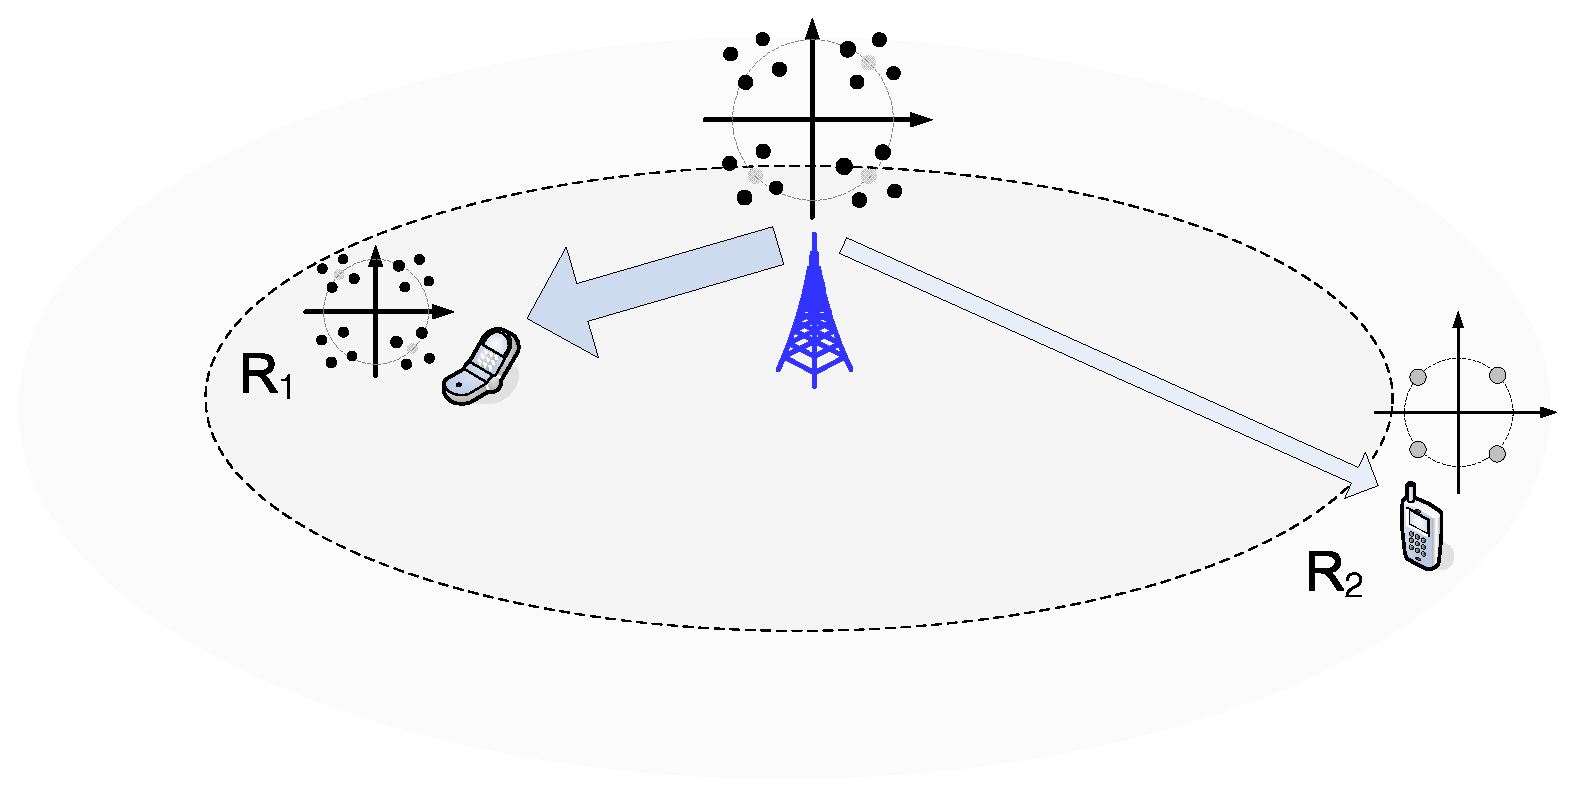
\includegraphics[width=3.50in, angle=0]{BC_Model.eps}
\caption{A broadcast channel model with two coverages and the
enhanced QPSK/QPSK hierarchical modulation.}\label{BC} }
\end{figure}
Instead of the traditional single-coverage broadcast network, a
broadcast channel model with two coverages is considered here and
it is illustrated in Fig.~\ref{BC}. In this model, the broadcast
station (BS) transmits signals to all mobile stations (MS)in the
covered area. The MS's located near to the edge may only reliably
decode the data stream of a low rate $R_1$ while the MS's close to
BS can reliably decode the data stream of a high rate $R_2$. For
achieving this, hierarchical modulation is employed so that the
modulated symbol streams can be taken as two synchronously
superposed symbol substreams. The rationale behind it is the
result from broadcast channel capacity theory, which states that
with superposition precoding (SPC), a little sacrifice on the rate
for the users near to the edge can lead to a big rate increase for
the users with good reception condition. This can be illustrated
in Fig.~\ref{SPC}. And hierarchical modulation can be taken as a
practical implementation of SPC.
\begin{figure}
\center{
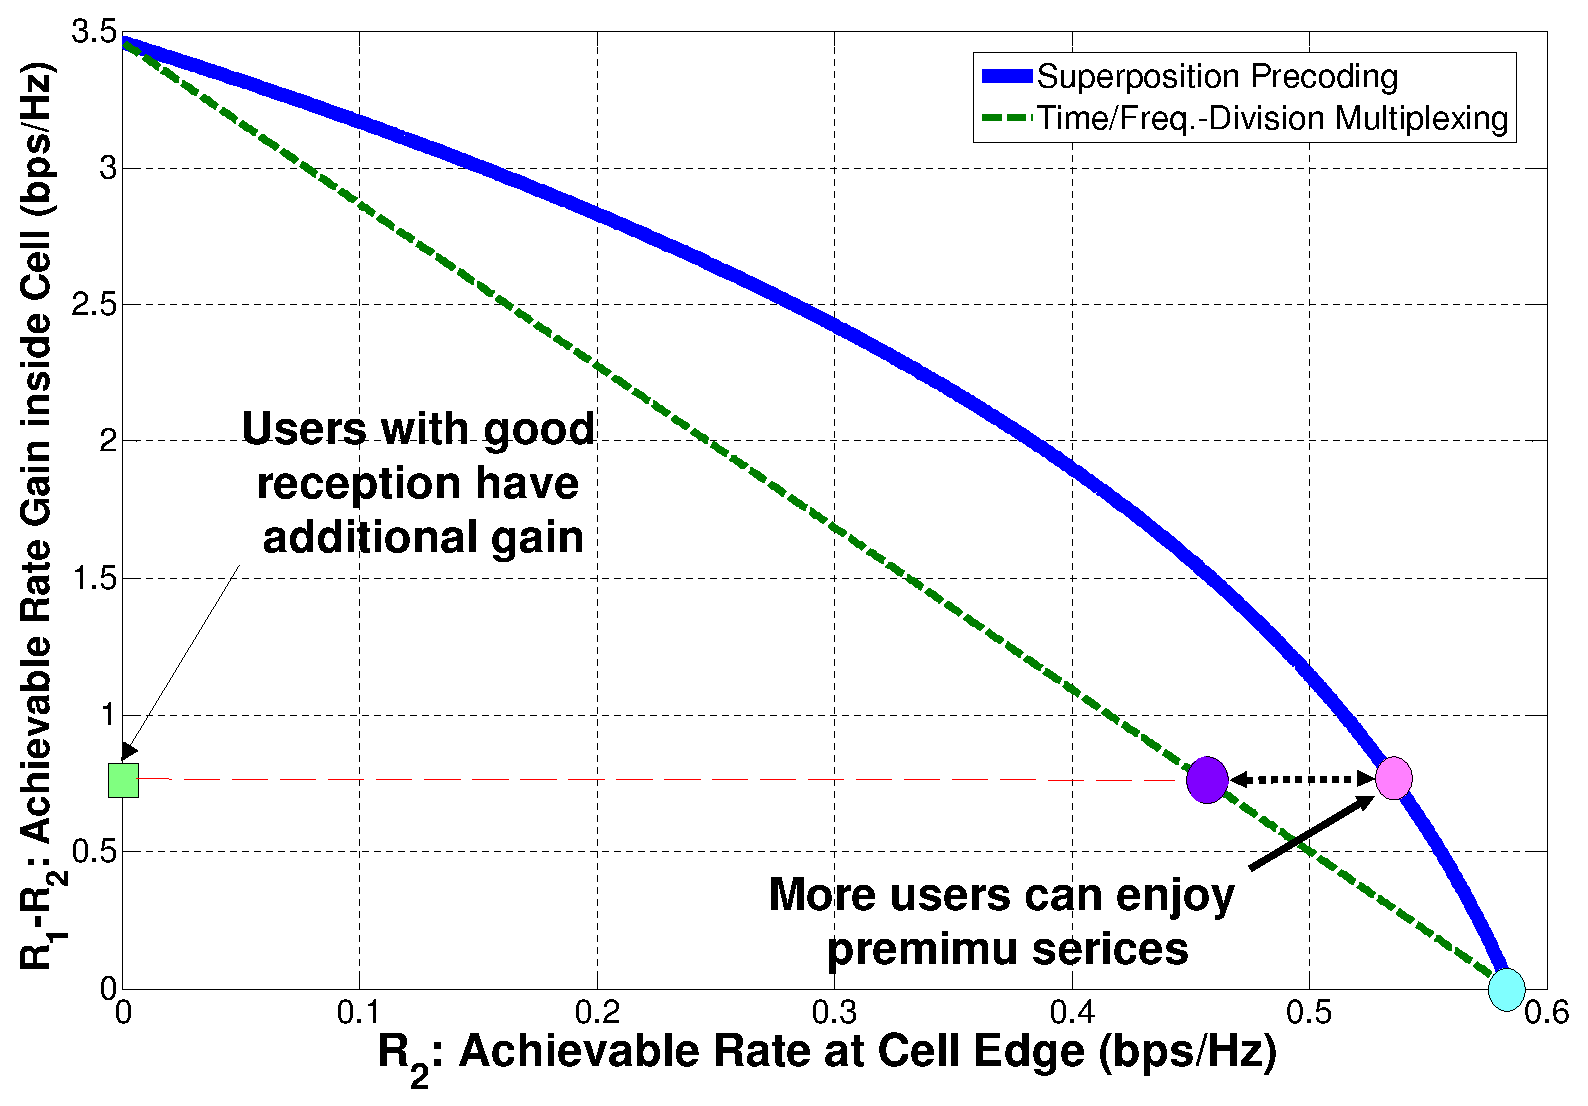
\includegraphics[width=3.50in, angle=0]{SPC.eps}
\caption{Achievable capacity region of broadcast
channel.}\label{SPC} }
\end{figure}

\subsection{Hierarchical Modulation and Inter-Layer Interference}
The signal constellations of regular square-shaped QPSK/QPSK and
16QAM/QPSK hierarchical modulation are shown in Fig.
\ref{regular_hierarchical}~\footnote{In this paper, a hierarchical
modulation is denoted by {\em layer 0 (or base layer)
constellation / layer 1 constellation / \ldots}, where the signal
constellation of different layers are separated by backslash from
the lowest layer (also called base layer ) to the highest layer.
}. Obviously, the regular 16QAM can be taken as a special case of
QPSK/QPSK hierarchical modulation, in which both base layer and
enhancement layer are QPSK-modulated. The minimum Euclidean
distance (MED) of base layer and enhancement layer are denoted by
$2\alpha$ and $2\beta$, respectively~\footnote{Without loss of
generality, it is assumed that $\alpha\geq\beta$ in most cases.}.
With superimposing base-layer signal and enhancement layer signal
together, the MED of resulted hierarchical modulation becomes
\begin{equation}
\begin{array}{rcccl}
d_{\rm min}& = & \min\left\{2\left(\alpha-\beta\right),\ 2\alpha,\
2\beta\right\}&<& 2\alpha
\end{array}.\label{Regular_MED}
\end{equation}
\begin{figure}
\center{
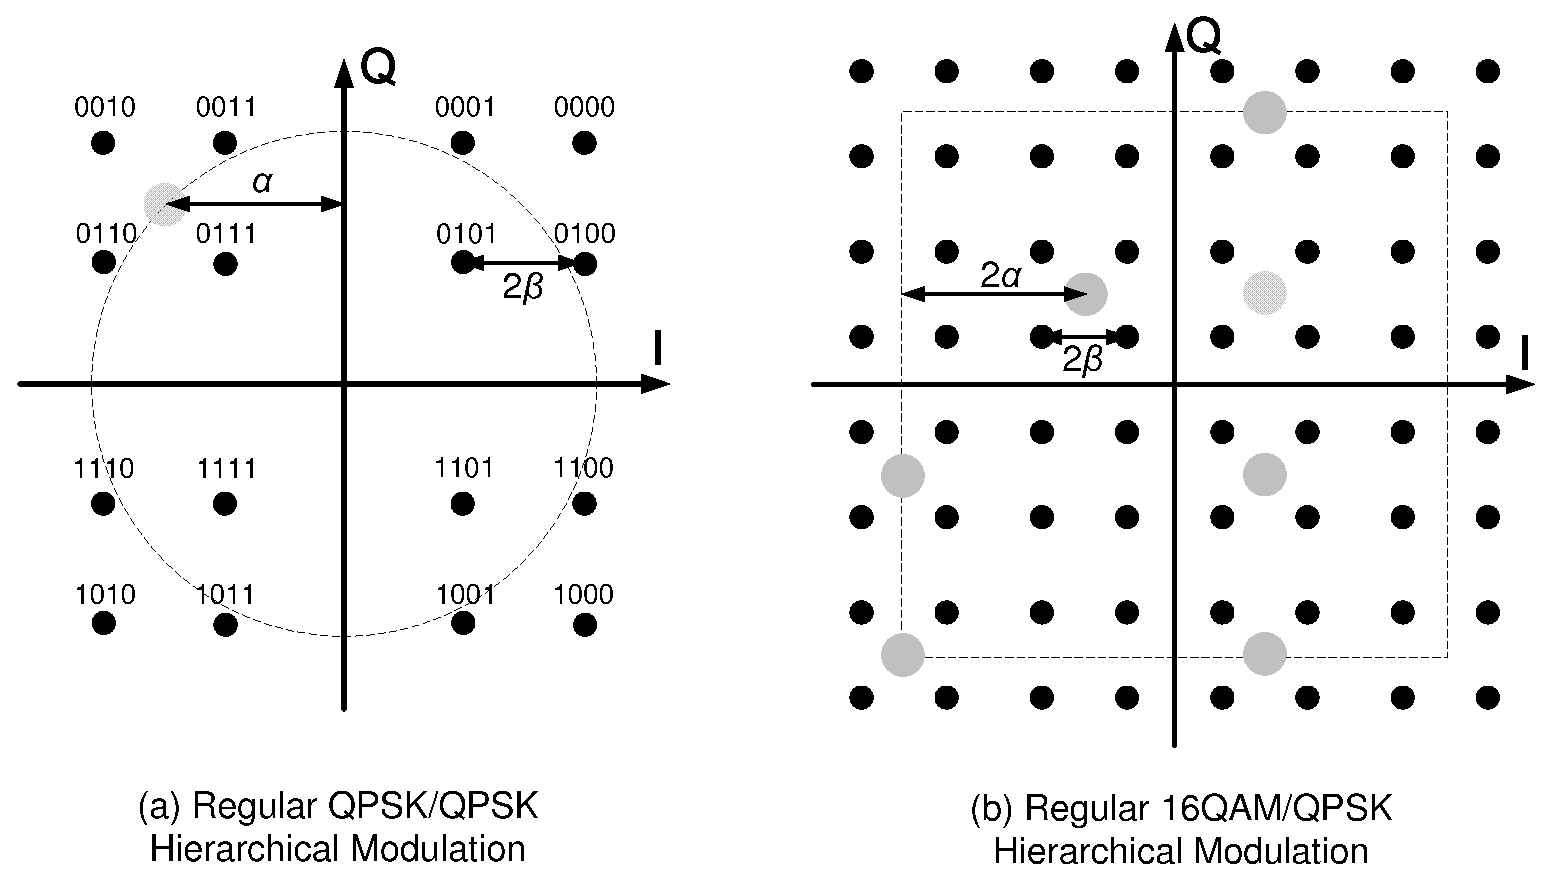
\includegraphics[width=3.0in, angle=0]{Regular_Hierarchical.eps}
\caption{Regular hierarchical modulation examples: the base layer
is QPSK/16QAM and the enhancement layer is
QPSK.}\label{regular_hierarchical} }
\end{figure}
\noindent Smaller minimum Euclid distance usually results in more
ambiguity and more demodulation errors. And the power-splitting
ratio $\zeta$ between layers is defined by
\begin{equation}
\begin{array}{rcl}
\zeta & = & \frac{P_{\rm E}}{P_{\rm B}}
\end{array}\label{power_ratio}
\end{equation}
\noindent with $\zeta < 1$ in most cases. For QPSK/QPSK
hierarchical modulation, the power-splitting ratio is
$\zeta_{\mbox{\tiny QPSK/QPSK}}= \frac{\beta^{2}}{\alpha^2}$. For
16QAM/QPSK modulation, $\zeta_{\mbox{\tiny 16QAM/QPSK}}=
\frac{\beta^{2}}{4\alpha^2}$. When $\zeta_{\mbox{\tiny
QPSK/QPSK}}=\frac{1}{4}$, the QPSK/QPSK modulation in
Fig.~\ref{regular_hierarchical}(a) becomes square-shaped 16QAM. In
general, the enhancement-layer signal can be taken as additional
noise by base layer. At this time, most existing conventional
receivers can continue to demodulate base-layer signals with no
additional change but at a lower signal-to-noise/interference
ratio (SINR) $\hat{\gamma}$ defined by
\begin{equation}
\begin{array}{rcccccl}
\hat{\gamma}& = & \frac{P_{\rm B}}{P_{\rm
E}+\sigma^2}&<&\gamma&=&\frac{P_{\rm B}}{\sigma^2}
\end{array}\label{SINR}
\end{equation}
\noindent with the background additive Gaussian white noise (AWGN)
power $\sigma^2$,  especially when $\zeta$ is small. On the other
hand, signals of both base layer and enhancement layer(s) can also
be demodulated by a advanced receiver. This is the strictly
backward compatibility of hierarchical modulation, which makes it
attractive for providing seamless upgrading with little change on
existing digital broadcast systems.


Though the schemes proposed here can straightforwardly be
generalized for most hierarchical modulations and multicarrier
transmission schemes, our discussions will be limited to two-layer
signal constellations over OFDM with QPSK-modulated enhancement
layer and QPSK- or 16QAM-modulated base layer in this paper. The
reason for this is not only because of the simplicity of QPSK and
16QAM modulations over OFDM but also because QPSK and 16QAM as
well as OFDM are of the most popular signal constellations and
transmission schemes adopted in various digital communication
systems and standards. It is shown that the use of QPSK as
enhancement layer can yield significant performance gain with our
approaches. On the other hand, many high-order regular or
hierarchical signal constellations may be decomposed into multiple
QPSK signals adding together and most results for OFDM can be
applied to other multicarrier transmission.

\subsection{Orthogonal Frequency-Division Multiplex and Peak-to-Average-Power Ratio}

An OFDM signal is the sum of $L$ independent modulated symbols
$\left\{s_{l}:\ 1\leq l\leq L\right\}$ mapped onto $L$ different
subcarriers with the frequency separation $\frac{1}{T}$, where $T$
is the symbol period with no additional overhead such as cyclic
prefix (CP) and zero prefix (ZP). At the transmitter side, the
discrete time-domain samples $\left\{x_{m}:\ 1\leq m\leq
L\right\}$ are the inverse fast Fourier transform (IFFT) of the
complex symbols $\left\{s_{l}:\ 1\leq l\leq L\right\}$:
\begin{equation}
\begin{array}{lcl}
x_{m}&=&\frac{1}{\sqrt{L}}\sum\limits_{l=0}^{L-1}s_{l}e^{j2\pi\frac{ml}{L}}
\end{array}.\label{OFDM}
\end{equation}
\noindent Before transmission, $x_{m}$ is usually extended by
attaching a CP or ZP. When CP is applied, the extended OFDM symbol
\begin{equation}
\begin{array}{rcl}
\tilde{x}_{n}&=&\Bigg\{ \begin{array}{ll}x_{n}&1\leq n\leq L\\
x_{n+L}&-L_{cp}+1\leq n\leq 0 \end{array}
\end{array}.
\end{equation}
\noindent The extended OFDM symbol then passes through
digital-to-analog converter and pulse-shaping filter before
up-converted to the carrier frequency. The PAPR of OFDM signal is
usually defined by
\begin{equation}
\begin{array}{rcl}
\xi&=&\frac{1 }{\mbox{E}\left\{\left|x_{m}\right|^2\right\}
}\max\limits_{m} \left|x_{m}\right|^{2}
\end{array},
\end{equation}
\noindent though in practice the PAPR of the analog signal
equivalent of $\left\{\tilde{x}_{n}:\ -L_{cp}+1\leq n\leq
L\right\}$ is more of interest.

\section{The Enhanced Hierarchical Modulation}
\begin{figure}
\center{
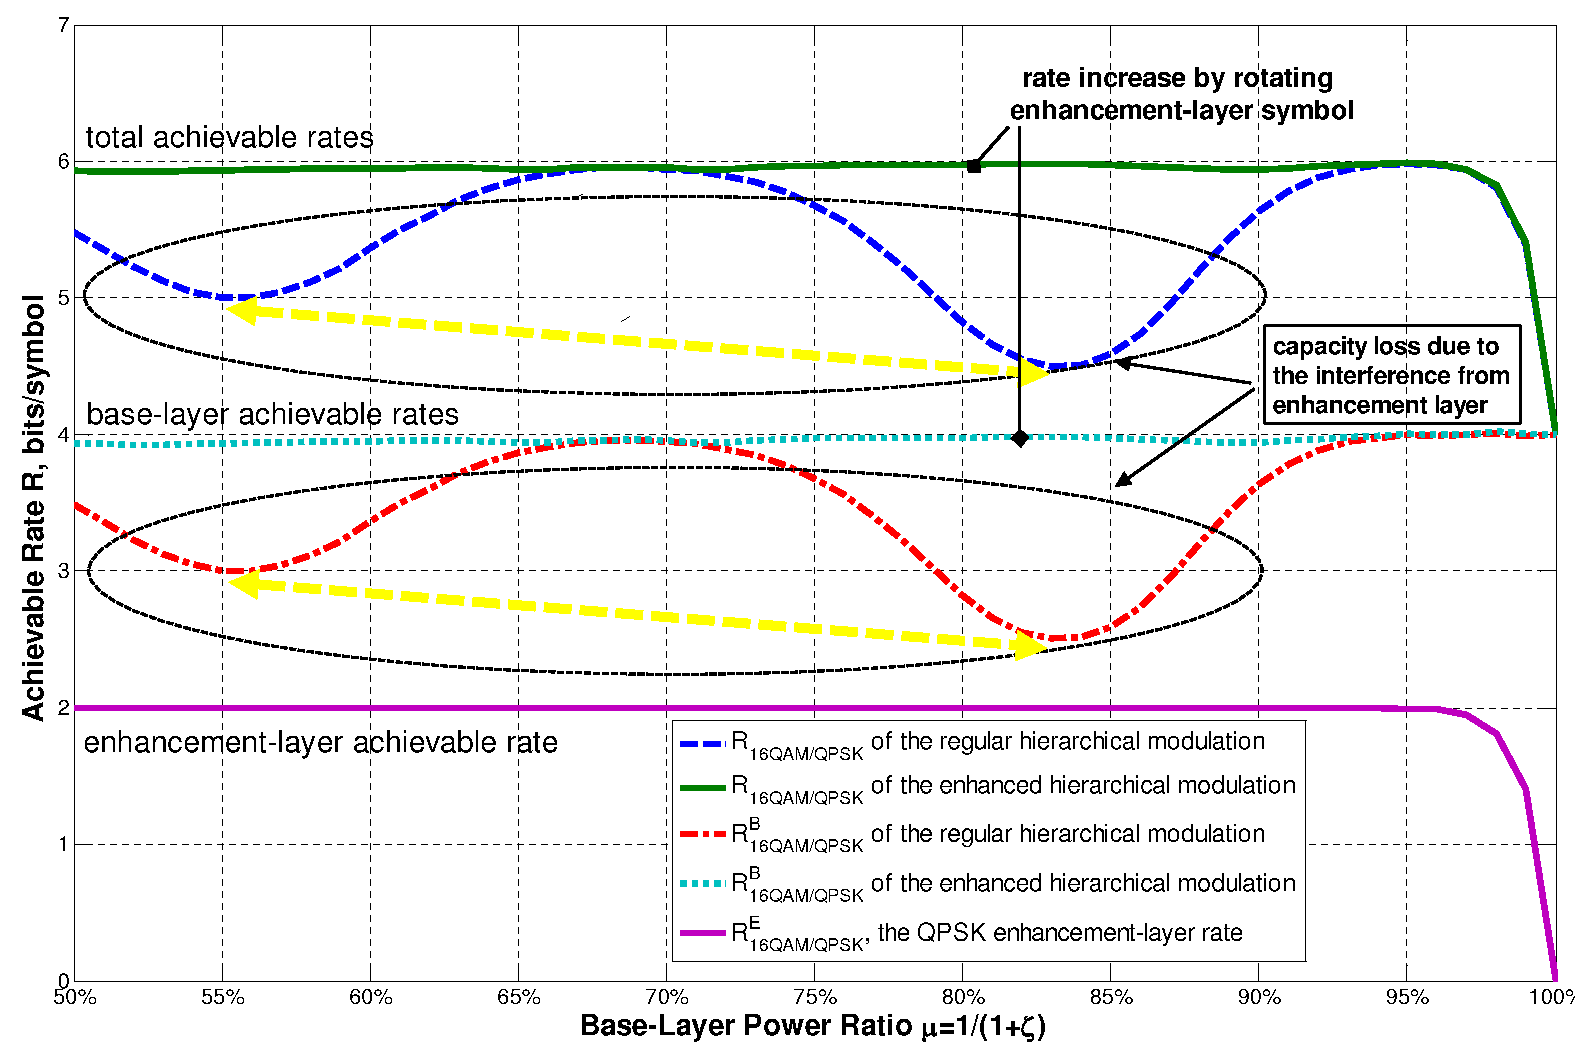
\includegraphics[width=3.0in, angle=0]{Capacity_power_splitting.eps}
\caption{Achievable rates of 16QAM/QPSK hierarchical modulation
with different power splitting and
$\frac{P}{\sigma^2}=20$dB.}\label{capacity_rotating} }
\end{figure}

Regular hierarchical modulation may seriously suffer from ILI,
which not only decreases the base-layer SINR from ${\gamma}$ to
$\hat{\gamma}$ but also lowers the achievable spectral efficiency.
This is observed from Fig.~\ref{capacity_rotating}. It is
well-known that the achievable throughput of a hierarchical
modulated signal essentially depends on the power distribution
profile of the signal~\cite{Unge82} in signal space. This somehow
is similar to channel coding. From a channel coding point of view,
higher throughput is achievable by the {\em i.i.d. Gaussian code}
defined in coding space, even though it may not be implementable
from an engineering standpoint~\cite{Cover72}. How to transmit a
signal close to Shannon channel capacity and implementable in a
relatively easy way is not only critical for the signal
constellation design but also every other component in a
communication system, including modulating signals.

In order to increase channel capacity with minimum complexity
increase, an enhancement modulation scheme is proposed to optimize
the signal constellation of hierarchical modulation for improving
the spectral efficiency, decreasing demodulation BER and
increasing transmission power efficiency. For these, we propose to
optimally rotate the enhancement-layer(s) of a signal
constellation. For the QPSK/QPSK hierarchical modulation shown in
Fig.~\ref{regular_hierarchical}(a), the QPSK signal constellation
of the enhancement layer is rotated in counter-clockwise by
$\theta$, $0\leq\theta\leq\frac{1}{4}\pi$, and resulted signal
constellation is shown in Fig. \ref{enhanced_hierarchical}(a). For
16QAM/QPSK, the regular and enhanced hierarchical modulations are
shown in Fig.~\ref{regular_hierarchical}(b) and Fig.
\ref{enhanced_hierarchical}(b), respectively.  As shown in
Fig.~\ref{capacity_rotating}, with optimal rotation angle
$\theta_{\rm opt}$, most of the lost base-layer capacity can be
recovered without scarifying the throughput of enhancement
layer(s) and the achievable rate of QPSK-modulated enhancement
layers is unchanged before and after the rotation.
\begin{figure}
\center{
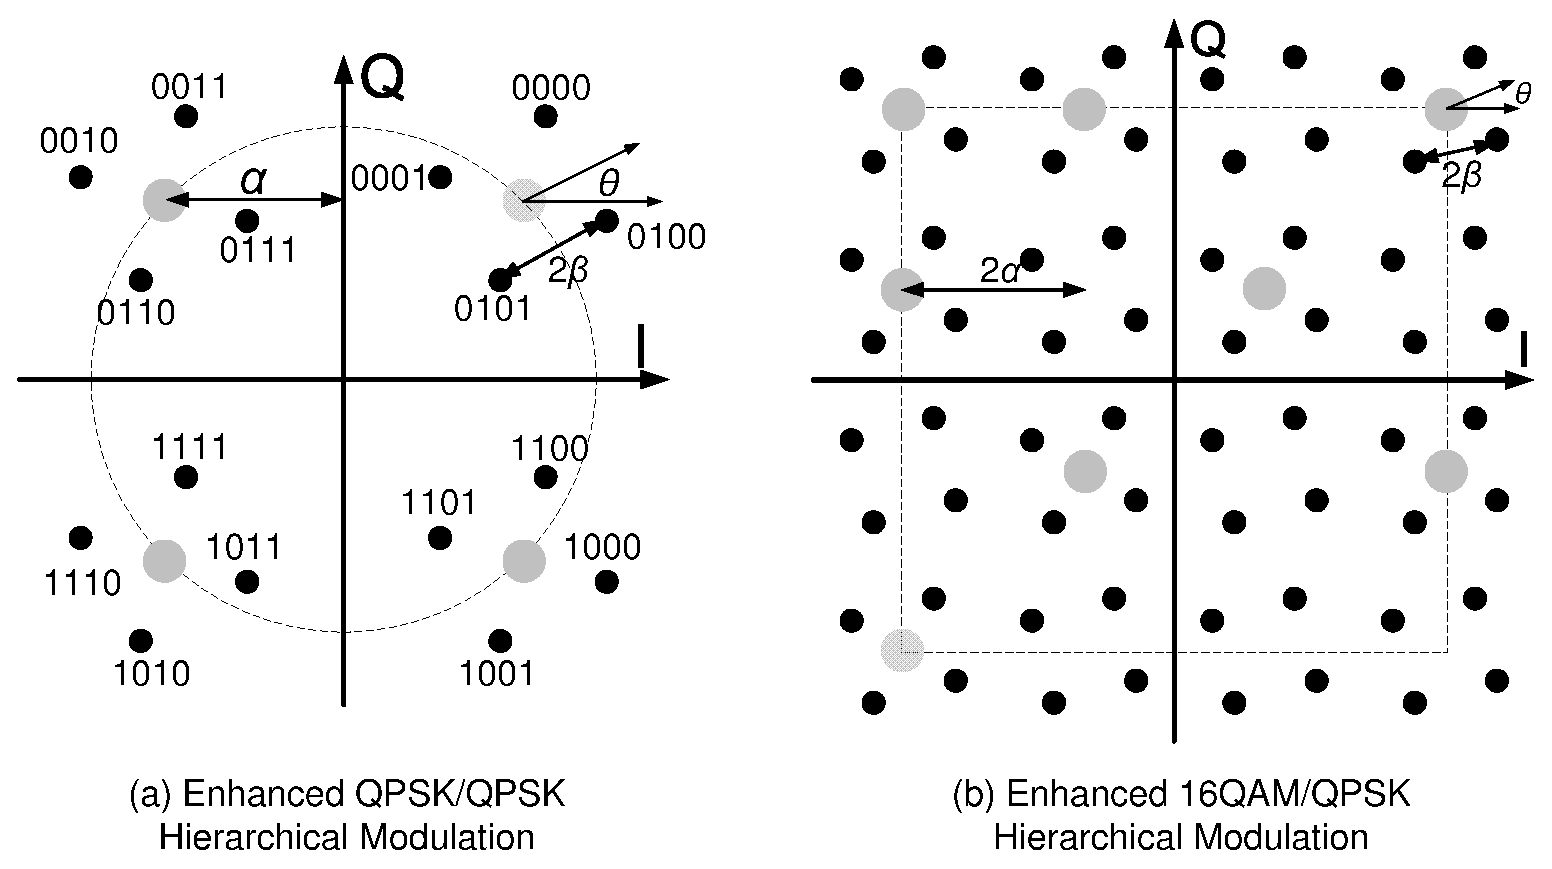
\includegraphics[width=3.0in, angle=0]{Enhanced_Hierarchical.eps}
\caption{Enhancing hierarchical modulation by
rotation.}\label{enhanced_hierarchical} }
\end{figure}

\section{Optimizing Hierarchical Modulation}

\subsection{Maximizing Achievable Rates~\label{Info_Theory}}

More three decades ago Cover showed that higher sum capacity is
achievable if messages for two users of different receptions are
superposited~\cite{Cover72}. Hierarchical modulation is one of the
practical implementations of superposition precoding (SPC) for
providing different rates and protections to users. In general,
the achievable rate of a $N$-ary modulated signal, of either
regular or hierarchical signal constellation, through AWGN channel
is given by~\cite{Unge82}
\begin{equation}
\begin{array}{lcl}
R&=&\log_{2}\left(N\right)-\\
&&\hspace{-0.20in}\frac{1}{N}\sum\limits_{i=0}^{N-1}\mbox{E}\left\{\log_{2}\left[\sum\limits_{j=0}^{N-1}e^{-\frac{\left|s_{j}+n-s_{i}\right|^2-\left|n\right|^2}{2\sigma^2}}\right]\right\}\
.
\end{array}\label{N_ary}
\end{equation}
\noindent This is the achievable rate when a receiver try to
decode the whole hierarchically modulated symbol. With
(\ref{N_ary}), the AWGN capacity of regular QPSK and 16QAM can be
plotted in Fig \ref{capacity_16QAM}. Though the rate in
(\ref{N_ary}) is achievable by users with advanced receiver, it is
more than achievable for a user with a conventional receiver which
usually detects the base-layer signals only. The achievable rate
of either base layer or enhancement layer is lower than the total
rate in (\ref{N_ary}). Following the concept of the successive
interference cancellation, the achievable rate, also termed {\em
equivalent capacity}, for a receiver decoding up to $l$ layers of
a hierarchical modulated symbol is~\cite{Huber94}
\begin{equation}
\begin{array}{rcccl}
\tilde{R}_{l}&=&\sum\limits_{i=0}^{l-1}R_{i}& = &
R-\sum\limits_{j=l}^{L}{R}_{j}
\end{array}.\label{R_equiv}
\end{equation}
\noindent To illustrate this, let's take the regular 16QAM as an
example since a regular 16QAM can be take as a special case of
QPSK/QPSK hierarchical modulation with $\zeta_{\mbox{\tiny
QPSK/QPSK}}=\frac{1}{4}$. This means the achievable rate of the
enhancement layer is the same as the regular QPSK capacity but the
achievable rate of the QPSK base layer becomes
\begin{equation}\hspace{-0.2in}
\begin{array}{rl}
{\rm R}_{\mbox{\tiny QPSK/QPSK}}^{\rm B}\left(\gamma,\
\frac{1}{5}\right)&\hspace{-0.08in}=\ {\rm R}_{\mbox{\tiny
QPSK/QPSK}}\left(\gamma,\
\frac{1}{5}\right)-{\rm R}_{\mbox{\tiny QPSK}} \left(\frac{1}{5}\gamma\right)\\
&\hspace{-0.08in}=\ {\rm R}_{\mbox{\tiny
16QAM}}\left(\gamma\right)-{\rm R}_{\mbox{\tiny
QPSK}}\left(\frac{1}{5}\gamma\right)\ .
\end{array}\label{R_16QAM_B1}
\end{equation}
\noindent They are plotted in Fig \ref{capacity_16QAM}. Due to the
ILI from the QPSK-modulated enhancement layer, the actual
throughput of the QPSK base layer ${\rm R}_{\mbox{\tiny
QPSK/QPSK}}^{\rm B}\left(\gamma,\ \frac{1}{5} \right)$ is lower
than the corresponding QPSK rate ${\rm R}_{\mbox{\tiny
QPSK}}\left(\frac{4}{5}\gamma\right)$, i.e.,
\begin{equation}
\begin{array}{rcl}
{\rm R}_{\mbox{\tiny QPSK/QPSK}}^{\rm B}\left(\gamma,\ \frac{1}{5}
\right)&\leq&{\rm R}_{\mbox{\tiny QPSK}}
\left(\frac{4}{5}\gamma\right)
\end{array}.\label{R_16QAM_B2}
\end{equation}
\begin{figure}
\center{
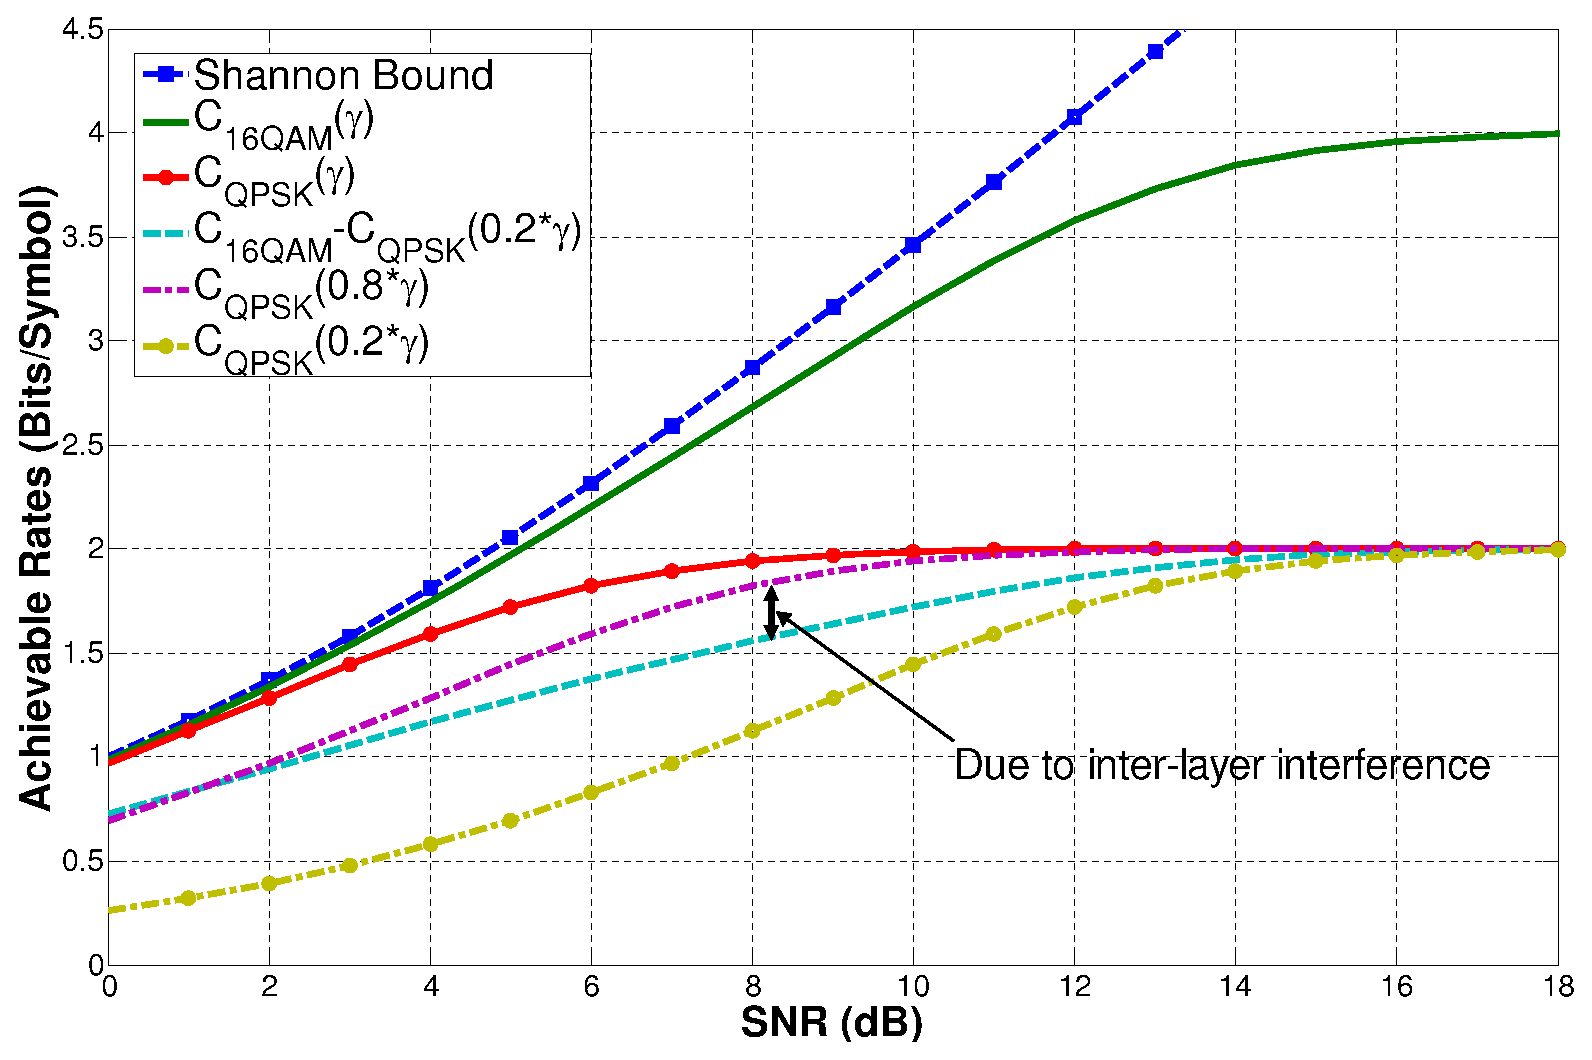
\includegraphics[width=3.0in, angle=0]{Capacity_16QAM.eps}
\caption{Achievable rates of regular 16QAM modulation: a
hierarchical modulation perspective.}\label{capacity_16QAM} }
\end{figure}
\noindent In Fig \ref{capacity_16QAM}, it shows that the
degradation of the base-layer capacity can be up to around
$\Delta=0.56$ bits/symbol, which is about $14\%$ of the maximum
total achievable rate $2$ bits/symbol for the QPSK base-layer.
This kind of degradation can be further illustrated in
Fig.~\ref{capacity_rotating}, where the hierarchical modulation is
16QAM/QPSK-modulated. In Fig.~\ref{capacity_rotating}, the total
SNR is fixed at $\frac{P}{\sigma^2}=20\mbox{dB}$ but the power of
the 16QAM sublayer is changed from $50\%$ to $100\%$ of the total
power $P$. The achievable rates of each layer and the whole signal
constellation are plotted in Fig.~\ref{capacity_rotating}. One of
the interesting things shown in Fig. \ref{capacity_rotating} is
the equivalent capacity of the 16QAM base layer changes
periodically instead of monotonically with increase the power
ratio of the base layer. The good things in Fig.
\ref{capacity_rotating} is this kind of capacity loss can be
recovered by optimally rotating the enhancement layer. This is one
of the advantages of the proposed enhanced hierarchical
modulations.

\subsection{Maximizing Modulation Efficiency}

Besides the above information-theoretical point of view on
hierarchical modulation, it is also interesting to understand
hierarchical modulation from a practical signal-processing
perspective. At this time, the performance of hierarchical
modulation will be evaluated through actual implementations, where
demodulation BER is one of the major concerns. In general, it is
difficult to give a simple closed-form BER expression for
hierarchical signal constellation, which also depends on receiver
design. The BER of square-shaped $M$-QAM constellation and a
hierarchical QAM constellation for maximum likelihood (ML)
demodulator can be computed by using recursive
algorithms~\cite{Vitt03}. It is known that the BER expression for
QPSK is
\begin{equation}
\begin{array}{rcl}
{\rm P}_{e,\mbox{\tiny QPSK}}\left(\gamma\right)&=&{\rm
Q}\left(\sqrt{\frac{\gamma}{2}}\right)
\end{array},\label{BER_QPSK}
\end{equation}
\noindent where ${\rm Q}\left(x\right)=\frac{1}{2}{\rm
erfc}\left(\frac{x}{\sqrt{2}}\right)$ denotes the $\rm
Q$-function.
\begin{figure} \center{
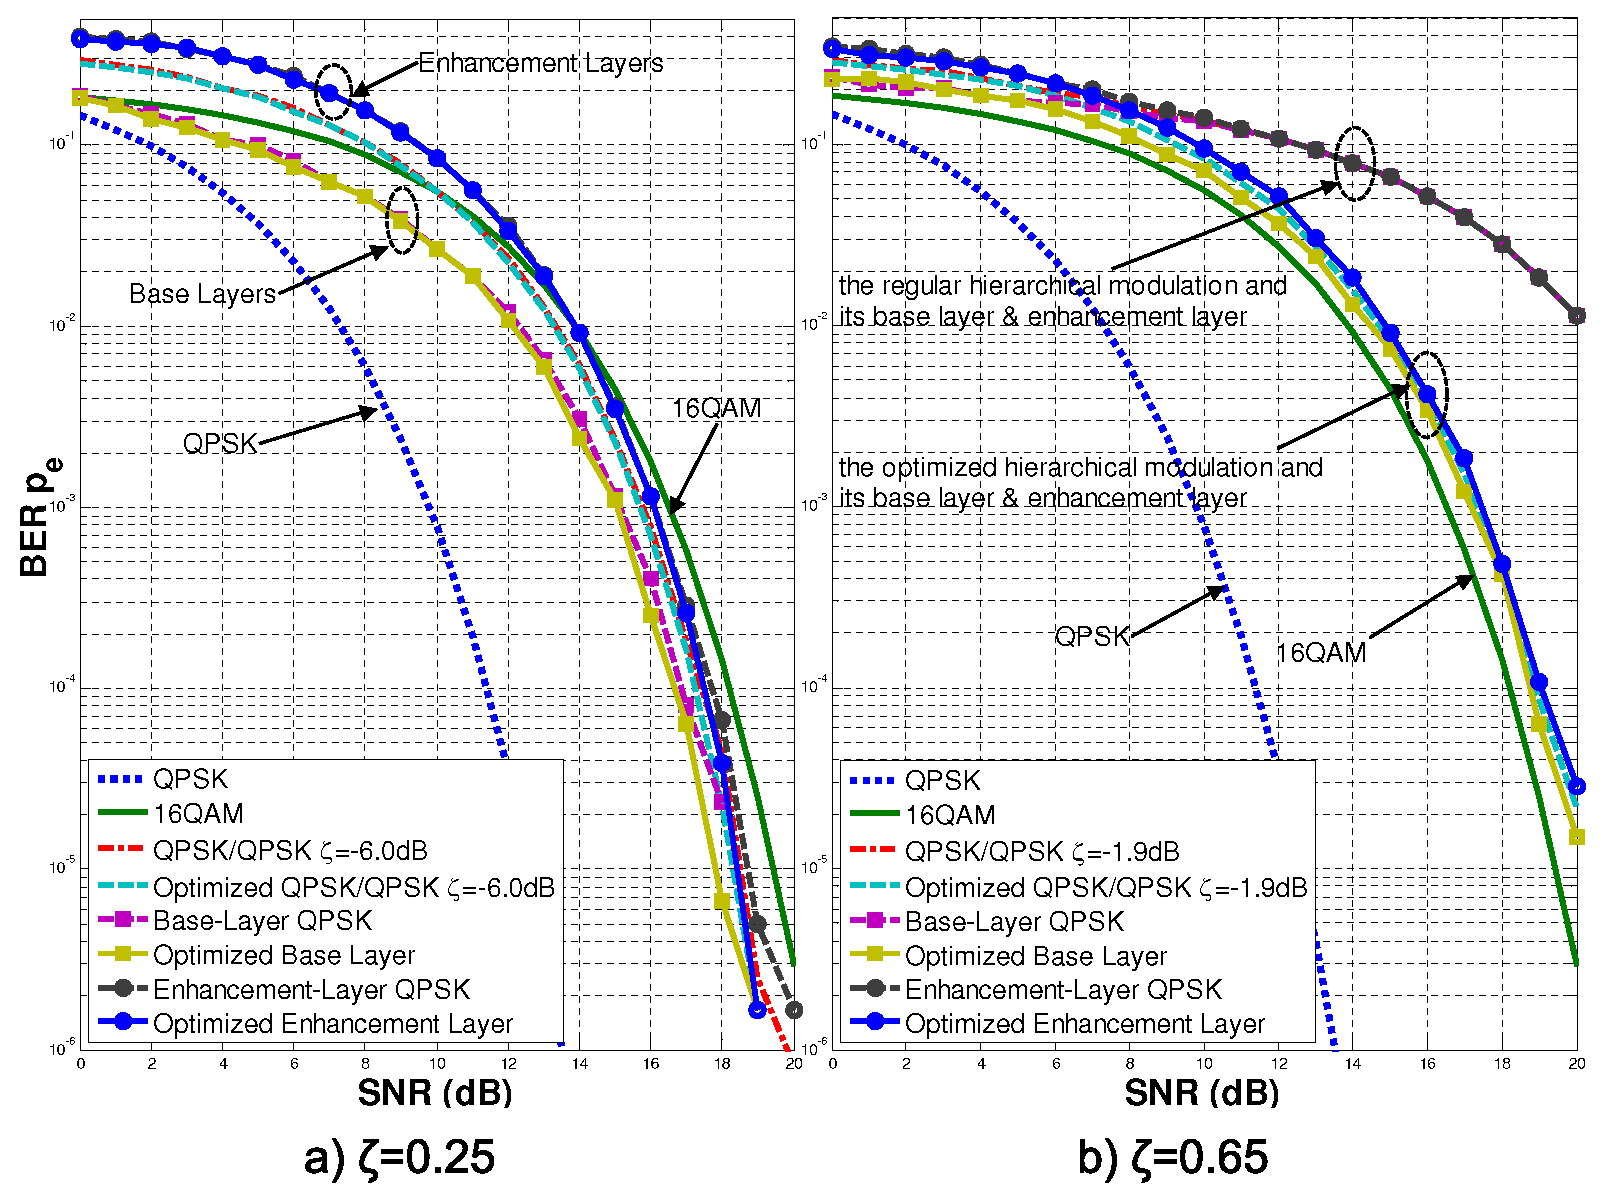
\includegraphics[width=3.20in, angle=0]{BER_Hierarchical.eps}
\caption{Bit-error rate of uncoded QPSK/QPSK hierarchical
modulations using maximum likelihood demodulation . } \label{BER}}
\end{figure}
From a signal processing standpoint, the BER and capacity
degradation may happen when there is a change in noise and/or
interference distribution, even though the received SNR $\gamma$
is the same. For example, the BER performance of regular QPSK/QPSK
becomes deteriorated in Fig. \ref{BER} when increase
$\zeta_{\mbox{\tiny QPSK/QPSK}}$. But, if we optimally rotate the
enhancement-layer signal constellation, the performance loss can
be recovered. This kind of recovery is more significant with large
$\zeta$. There are many ways for quantifying and understanding
this kind of BER performance loss due to interference and receiver
design. One approach for capturing this kind of degradation is to
calculate the effective signal-to-noise ratio (ESNR) on the
receiver output, which is defined by
\begin{equation}
\begin{array}{rcl}
\tilde{\gamma}\left(\gamma\right)&\equiv&\Psi^{-1}\left(p_{e}(\gamma)\right)
\end{array},\label{eff_SNR}
\end{equation}
\noindent where $p_{e}(\gamma)$ is the demodulation BER of the
signal with SNR $\gamma$, and $\Psi^{-1}\left(\ast\right)$ denotes
the inverse function of $\Psi\left(\cdot\right)$, the demodulation
error probability function with no ILI. For example, the ESNR for
the QPSK-modulated base layer or enhancement layer of any
hierarchical modulation can be calculated by
\begin{equation}
\begin{array}{rcl}
\tilde{\gamma}_{\mbox{\tiny QPSK/QPSK}}&=&2\left[{\rm
Q}^{-1}\left(p_{e}(\gamma)\right)\right]^2
\end{array}.\label{eff_SNR_QPSK}
\end{equation}
\noindent More specifically, the ESNR for the base layer of
regular QPSK/QPSK hierarchical modulation with ML demodulator is
given by
\begin{equation}\hspace{-0.225in}
\begin{array}{l}
\tilde{\gamma}_{\mbox{\tiny QPSK/QPSK}}^{\rm
B}(\gamma)=2\left[{\rm Q}^{-1}\left(\frac{{\rm
Q}((1-\sqrt{\zeta})\gamma)+{\rm
Q}((1+\sqrt{\zeta})\gamma)}{2}\right)\right]^2.
\end{array}\label{eff_SNR_QPSK_QPSK}
\end{equation}
\noindent By normalizing ESNR by $\gamma$, we can obtain
hierarchical modulation efficiency (ME) $\eta$ by
\begin{equation}
\begin{array}{rcccl}
\eta\left(\gamma\right)&=&\frac{\tilde{\gamma}}{\gamma}&=&\frac{1}{\gamma}\Psi^{-1}\left(p_{e}(\gamma)\right)
\end{array}.\label{mod_eff}
\end{equation}
\noindent With no interference, $\eta\left(\gamma\right)=1$;
otherwise, $\eta\left(\gamma\right)<1$. $\eta$ is also the measure
of inter-layer resistance for hierarchical modulation. Higher ME
is, stronger interference-resistance the signal has. As an
example, the ME of QPSK/QPSK hierarchical modulation are plotted
in Fig. \ref{modulation_efficiency}. We can see the enhanced
hierarchical modulation has higher ME than the regular modulation.
The difference is more obvious when $\zeta$ becomes large. This
means enhanced hierarchical modulation has stronger inter-layer
interference resistance than regular hierarchical modulation.
\begin{figure}
\center{
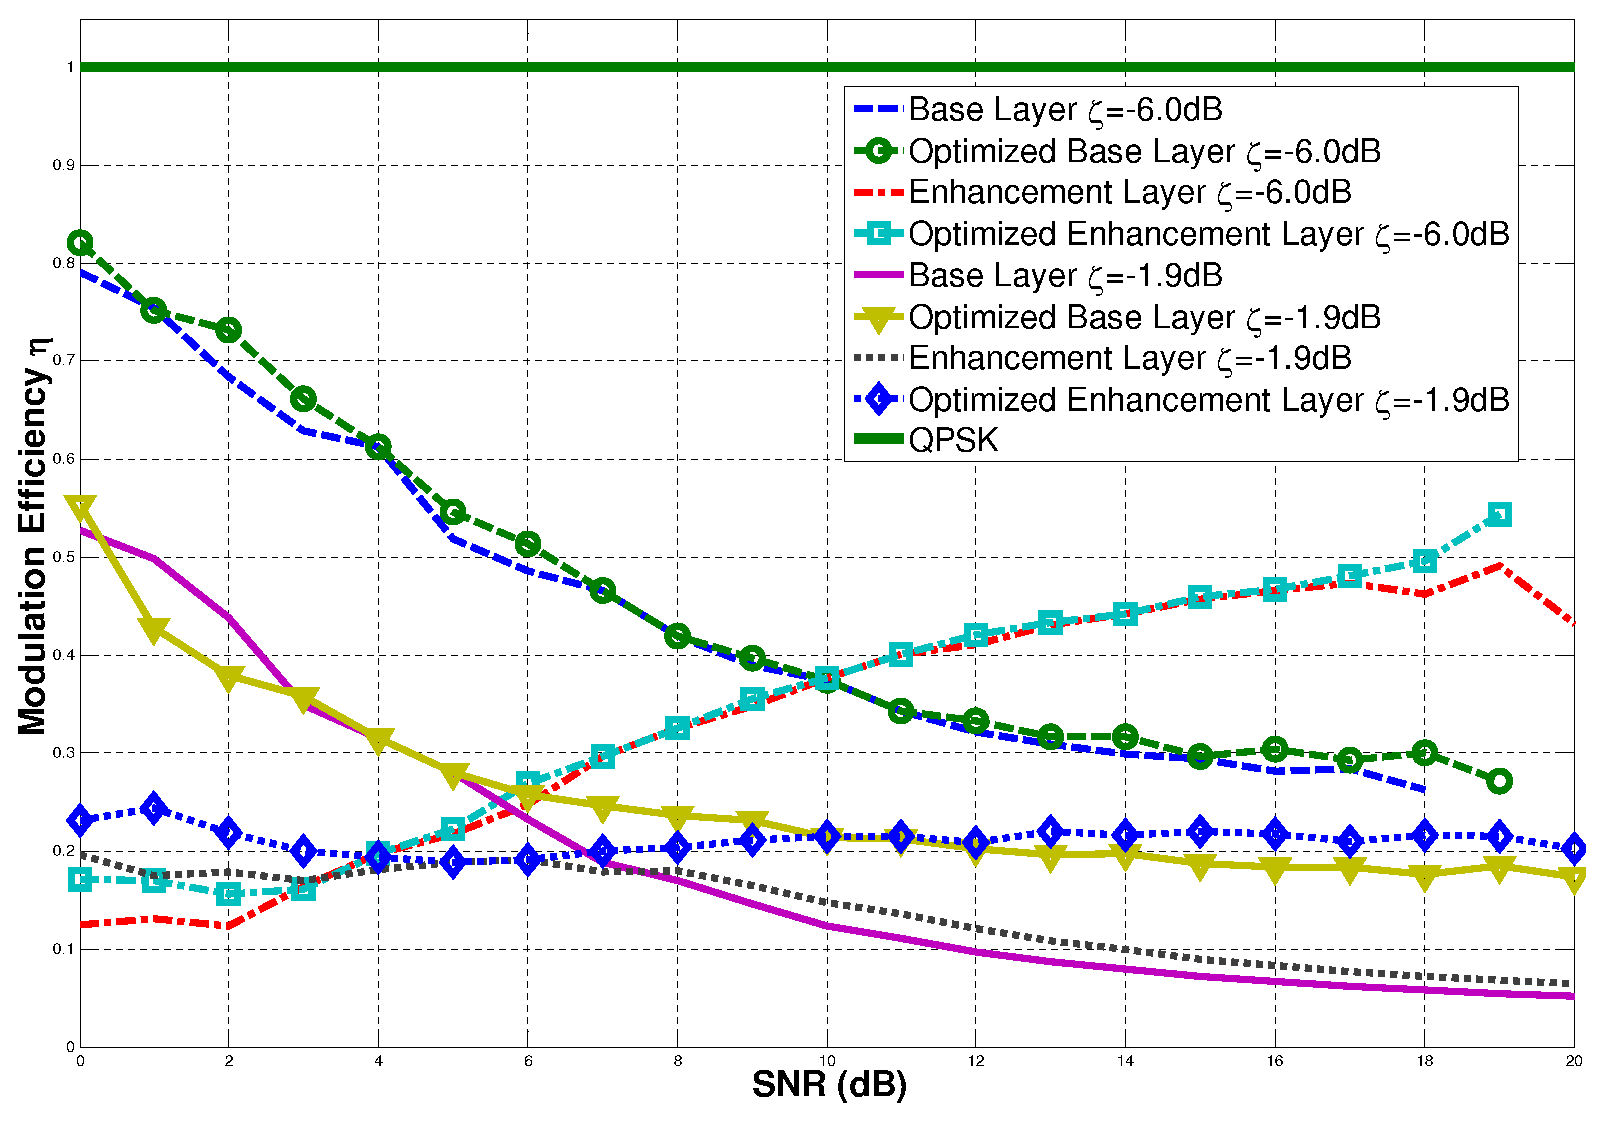
\includegraphics[width=3.0in, angle=0]{Modulation_Efficiency.eps}
\caption{Hierarchical modulation efficiency of QPSK/QPSK
hierarchical modulation using maximum likelihood
demodulation.}\label{modulation_efficiency} }
\end{figure}

The asymptotic modulation efficiency (AME) $\eta_{\infty}$ is
given by
\begin{equation}
\begin{array}{rcccl}
\eta_{\infty}&=&\lim\limits_{\gamma\rightarrow\infty}\eta\left(\gamma\right)&=&\lim\limits_{\sigma\rightarrow0}\frac{\sigma^2}{P}\Psi^{-1}\left(p_{e}\right)
\end{array}.\label{asy_mod_eff}
\end{equation}
\noindent For the example in (\ref{eff_SNR_QPSK_QPSK}), the AME
can be calculated by
\begin{equation}\hspace{-0.225in}
\begin{array}{rcl}
\eta_{\infty}&=&\lim\limits_{\gamma\rightarrow\infty}\frac{2\left[{\rm
Q}^{-1}\left(\frac{{\rm Q}((1-\sqrt{\zeta})\gamma)+{\rm
Q}((1+\sqrt{\zeta})\gamma)}{2}\right)\right]^2}{\gamma}.
\end{array}\label{asy_eff_SNR_QPSK_QPSK}
\end{equation}
\noindent From (\ref{asy_mod_eff}) and
(\ref{asy_eff_SNR_QPSK_QPSK}), it shows that AME basically shows
how fast ESNR is approaching SNR when $\gamma\rightarrow\infty$.
This can be expressed by
\begin{equation}
\begin{array}{rcl}
\eta_{\infty}&=&\frac{\partial\eta\left(\gamma\right)}{\partial\gamma}|_{\gamma=\infty}
\end{array}.\label{asy_mod_eff2}
\end{equation}
\noindent The AME for QPSK/QPSK hierarchical modulation can also
be found in Fig.~\ref{modulation_efficiency}, in which they are
the points approached when SNR becomes larger and larger.

\subsection{Minimizing Peak-to-Average-Power Ratio}
The RSSPA model of HPA is defined by
\begin{equation}
\begin{array}{rcl}
v_{\rm o}&=&\frac{v_{\rm i}}{\left[1+\left(\frac{|v_{\rm
i}|}{V_{\rm s}}\right)^{2K}\right]^{\frac{1}{2K}}}
\end{array},\label{RSSPA}
\end{equation}
\noindent where $v_{\rm i}$ and $v_{\rm o}$ respectively denote
the complex input and output signals, $V_{\rm s}$ denotes the
output saturation voltage level with $P_{\rm s}=\left|V_{\rm
s}\right|^2$ and $K$ denotes the knee factor, which controls the
smoothness of HPA characteristic.

\section{Conclusions}
In this paper, two schemes for enhancing hierarchical modulations
are presented for higher throughput and less error rate. One
approach is to optimize the signal constellation and the other one
is to optimize the bits-to-symbol mapping. The rationales as well
as the performance of the proposed approaches are analyzed. They
can be used for helping upgrade and design BCMCS systems with
minimum complexity increase. Some of them is adopted in the 3.5G
standard UMB by 3GPP2. \small
\bibliographystyle{unsrt}
\bibliography{Hierarchical_Modulation}
\end{document}
